\subsubsection{Kullback-Leibler Divergence}

The computations between years for a given topic give some waited results. Indeed, as you can see in figures \ref{KL-topic7} and \ref{KL-topic1}, the divergence between years is really small. Especially for the topic 'swiss politic' because the words that are present in this topic ('confédération', 'suisse', 'fédéral', ...) are words that are used every year. Thus, when a year approximate another one, this is almost perfect. There is just an exception for the years 1840 to 1848 that have difficulties to approximate other years. It is easily explicable because the swiss federal state was created in 1848 so the vocabulary for the 'swiss politic' was not exactly the same between 1840 and 1848.

For a more general topic like 'culture', we can observe the same behaviour that have the \emph{Kullback-Leibler} Divergence without using the topics (see section \ref{metrics}). Indeed, the vocabulary for 'culture' should increase over years, so years of the 19$th$ century have more difficulties to approximate the years of the 20$th$ century and it is not the case in the other direction.

We can also note that use \emph{Kullback-Leibler} divergence to date articles is not a good idea, due to the general plots with the topics.


\begin{figure}[h!]
    \begin{minipage}[b]{0.48\linewidth}
        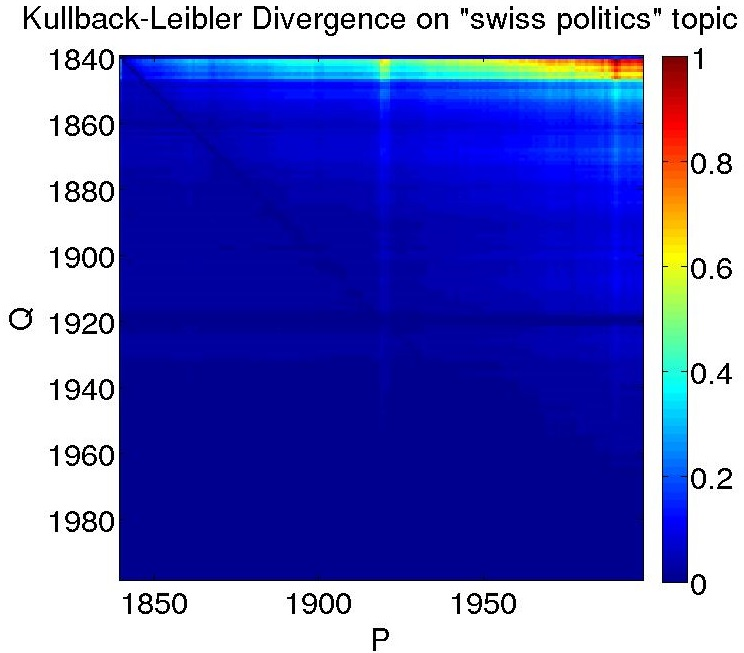
\includegraphics[scale=0.15]{Pictures/topics/kullback-leibler/KL_topic7.jpg}
        \caption{KL for the topic 'swiss politic'}
        \label{KL-topic7}
    \end{minipage}\hfill
    \begin{minipage}[b]{0.5\linewidth}
        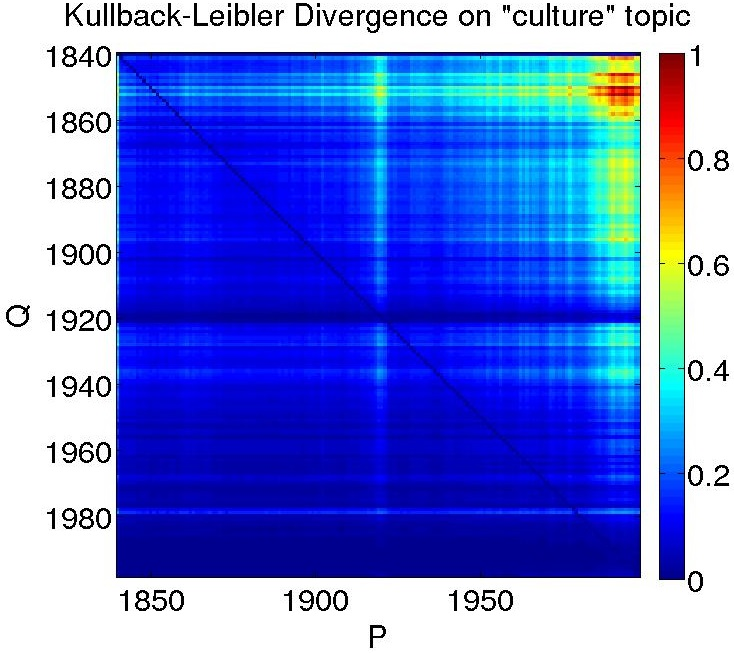
\includegraphics[scale=0.15]{Pictures/topics/kullback-leibler/KL_topic1.jpg}
        \caption{KL for the topic 'culture'}
        \label{KL-topic1}
    \end{minipage}\hfill
\end{figure}

Finally, for all the 15 topics that were extracted from the corpus, the divergence between years are well represented by the 2 examples in figures \ref{KL-topic7} and \ref{KL-topic1}. For topics that have vocabulary that not really changes over time, the divergence will be of the same kind as for the 'swiss politic' topic and and for the other it will be like the 'culture' topic.